\section{JSON}
JSON  (\emph{JavaScript Object Notation}) è un formato basato sul linguaggio
\emph{Javascript} utilizzato per lo scambio d'infomazioni in applicazioni
client-server. Attraverso la notazione JSON è possibile rappresentare qualsiasi
propietà di un oggetto, col vantaggio che la struttura del documento non è
vincolata a un modello prefissato, ma può variare nel tempo. Infatti è possibile
aggiungere e rimuovere proprietà dell'oggetto o addirittura modificarne il tipo
di dato rappresentato.
\\Un documento JSON è formato da due strutture:
\begin{itemize}
  \item Una collezione di coppie ``nome''/``valore'' ;
  \item Un elenco ordinato di valori. 
\end{itemize}
Un oggetto è una collezone non ordinata di coppie ``nome'' : ``valore''. Un
oggetto inizia con una parentesi graffa aperta ``\{`` e finisce con una parentesi
graffa chiusa ``\}''(Figura~\ref{fig:jsondoc}).
\begin{figure}[!h]
  \begin{center}
      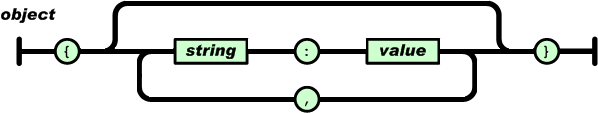
\includegraphics[scale=0.50]{jsondoc.png}
      \caption{Oggetto JSON}
      \label{fig:jsondoc}
  \end{center}
\end{figure}
\\Ogni nome di variabile è seguito dai due punti ``:'' e le coppie
``nome'' : ``valore'' sono separati
da una~virgola~``,''~(Figura~\ref{fig:jsonvalue}).
\begin{figure}[!h]
  \begin{center}
      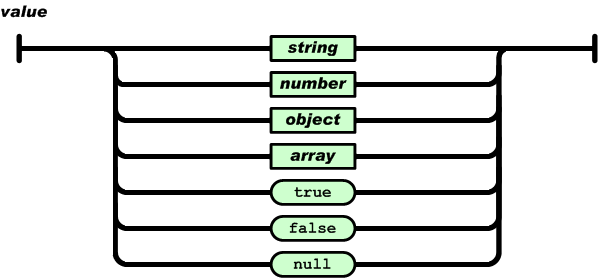
\includegraphics[scale=0.50]{jsonvalue.png}
      \caption{Valore di una variabile JSON}
      \label{fig:jsonvalue}
  \end{center}
\end{figure}
\\Un array è un insieme ordinato di valori. Un array comincia con una parentesi
quadra sinistra ``{[}'' e finisce con una parentesi destra``{]}''. I valori
sono separati da una~virgola~``,''~(Figura~\ref{fig:jsonarray}).
\begin{figure}[!h]
\begin{center}
    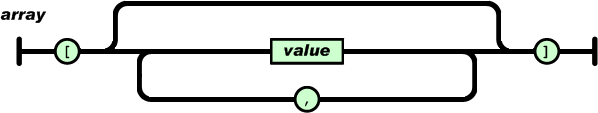
\includegraphics[scale=0.50]{jsonarray.png}
    \caption{Array JSON}
    \label{fig:jsonarray}
\end{center}
\end{figure}
\\\\\\L'oggeto utilizzato nel nostro modello è composto da sei variabili.
\emph{department} indica la facoltà per la quale è stata registrata una
votazione, il valore è una stringa univoca, nel caso la votazione si
riferisca ad un'operazione eseguita presso lo sportello veloce verrà registrata
con \emph{``sportello''}.\emph{Score} è una variabile numerica intera , nel
nostro modello può assumere i valori \{1,3,5\}.La data di effettuazione della
votazione,\emph{date} , viene raccolta dal sistema e salvata nel formato
``Y-m-d''.Gli attributi \emph{comment},\emph{customerName} e
\emph{customerEmail} nel caso il ciente lasci un feedback sono di tipo stringa , \emph{null} altrimenti. 
\\
\begin{lstlisting}[language=json] 
{ 
   _id:"182b00cd54a2b054fffabf1042000fbb", 
   _rev:"1-cb887f197900dce789c2dca898e4d330", 
   department: "engineering",
   score: 5,
   date: "2013-06-01T11:40:52.280Z",
   comment: "Ciao",
   customerName: "Alex Tomasello",
   customerEmail: null
}
\end{lstlisting} 
